\chapter{Diseño del simulador}
\label{chap:diseno_simulador}

En este capítulo se describe el diseño general del simulador desarrollado. Se presenta la arquitectura de la aplicación, el flujo de ejecución y la función de los principales componentes del sistema. Además, se explica cómo se organiza la interfaz de configuración, la escena de simulación, la integración entre Unity y Python, y la exportación de resultados.

\section{Arquitectura general del sistema}

La arquitectura general del simulador se divide en dos grandes bloques: la aplicación desarrollada en Unity y un entorno Python portable integrado. Unity actúa como base de la aplicación, encargándose de la interacción con el usuario, la configuración de la simulación, la construcción del escenario, la visualización de los resultados y la exportación final de datos. Por otra parte, Python se encarga de los cálculos relacionados con el canal de propagación y de la generación automática de gráficas.

En la Figura \ref{fig:arquitectura_general} se muestra el diagrama de componentes del sistema. En la parte superior se representa el bloque de Unity, formado por el menú de configuración, la escena de simulación y el cliente TCP. En la parte inferior se muestra el entorno Python portable integrado, que contiene el servidor TCP, el simulador Python y el generador de gráficas.

\begin{figure}[H]
    \centering
    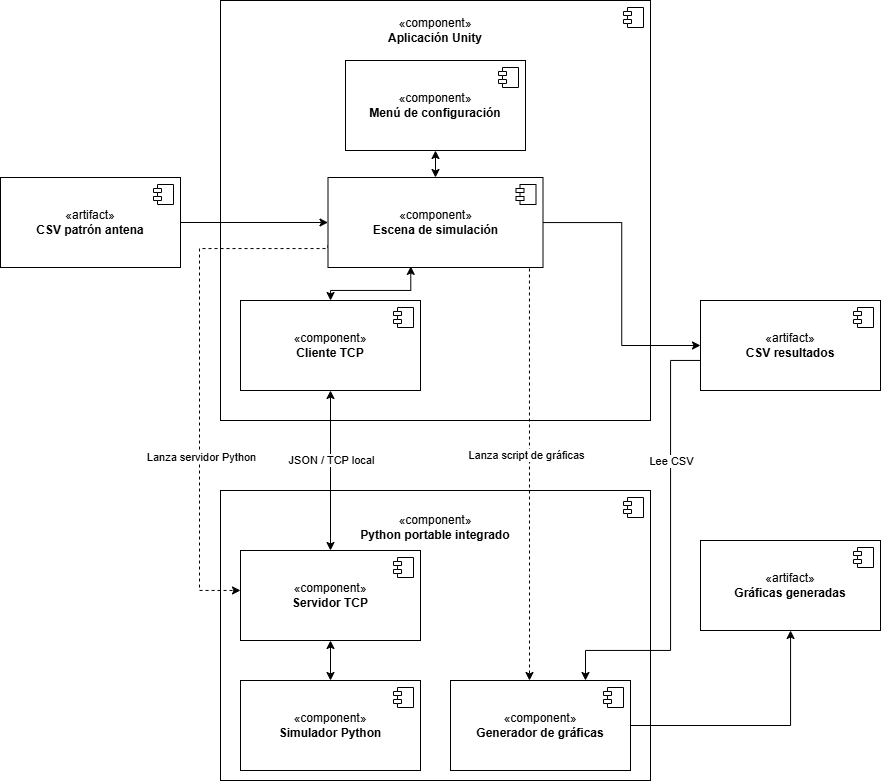
\includegraphics[width=1\textwidth, keepaspectratio]{imagenes/diagramas/Diagrama de componentes.png}
    \caption{Arquitectura general del simulador}
    \label{fig:arquitectura_general}
\end{figure}

Dentro de Unity, el menú de configuración permite introducir los parámetros necesarios para llevar a cabo la simulación, como la potencia de la antena transmisora, la frecuencia, el modelo de propagación o el tamaño de la rejilla que forma el mapa de calor tridimensional. Además, el sistema utiliza como entrada un fichero CSV con información del patrón de radiación de la antena. 

Este fichero contiene características básicas de la antena, junto con los valores del patrón de radiación en los planos horizontal y vertical. Con esta información, Unity reconstruye una aproximación tridimensional del patrón y calcula la ganancia de la antena en función de la dirección entre el transmisor y el punto del escenario deseado.

El entorno Python portable se integra dentro del proyecto para evitar depender de que el usuario final haya instalado Python previamente. Durante la simulación, Unity se comunica con un servidor TCP ejecutado en este entorno, enviando los datos necesarios y recibiendo los resultados calculados. Estos resultados se utilizan para representar la cobertura y generar los archivos de salida.

Con esta arquitectura se busca aprovechar lo mejor de cada entorno. Unity se utiliza para construir el escenario tridimensional, representar la cobertura y permitir que el usuario interactúe en tiempo real, mientras que Python permite reutilizar el simulador de propagación ya existente.

\section{Flujo de ejecución de la aplicación}

El funcionamiento de la aplicación se lleva a cabo a través de dos escenas principales: el menú de configuración y la escena de simulación. En el menú, el usuario ajusta los valores de los parámetros que se utilizarán posteriormente en la simulación. Estos pueden ser tanto técnicos, como la potencia de la antena transmisora, como visuales, de exportación o de rendimiento.

Antes de iniciar la simulación, la aplicación valida los datos introducidos. El usuario no puede avanzar hasta que todos los parámetros sean correctos. Cuando la configuración es válida, los parámetros se guardan y se carga la escena de simulación.

La Figura \ref{fig:flujo_general} muestra el flujo general de la aplicación. El bloque \textit{Ejecutar simulación} representa el proceso completo que se realiza dentro de la escena de simulación. Este proceso se explica en detalle en apartados posteriores de este capítulo.

\begin{figure}[H]
    \centering
    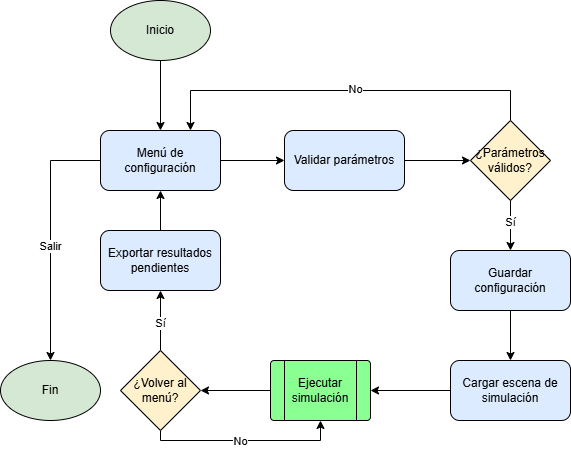
\includegraphics[width=1\textwidth, keepaspectratio]{imagenes/diagramas/Diagrama de flujo general.png}
    \caption{Flujo general de la aplicación}
    \label{fig:flujo_general}
\end{figure}

Durante la simulación, el usuario puede permanecer en la escena observando los resultados o volver al menú de configuración. En caso de volver al menú, la aplicación exporta los resultados pendientes para evitar que se pierda información. Además, desde el menú se puede cerrar la aplicación.

\section{Diseño del menú de configuración}

Una vez se inicia el simulador, el usuario puede elegir entre salir de la aplicación o iniciar la configuración. Desde este menú se ajustan todos los parámetros que se utilizarán posteriormente en la simulación, evitando que estos valores sean fijos o que deban introducirse manualmente a través de un fichero.

El menú está formado por una pantalla principal y cuatro pantallas de configuración. A su vez, estas pantallas se dividen en varias secciones. Esto hace que los parámetros queden organizados por bloques y la configuración sea más clara.

La Figura \ref{fig:diseno_menu} muestra la primera pantalla de configuración, dedicada a la antena y al modelo de propagación. En esta sección se encuentran algunos de los valores principales de la simulación, como la potencia de transmisión, la frecuencia, el ancho de banda, el modelo de pérdidas o el método utilizado para reconstruir el patrón de radiación de la antena.

\begin{figure}[H]
    \centering
    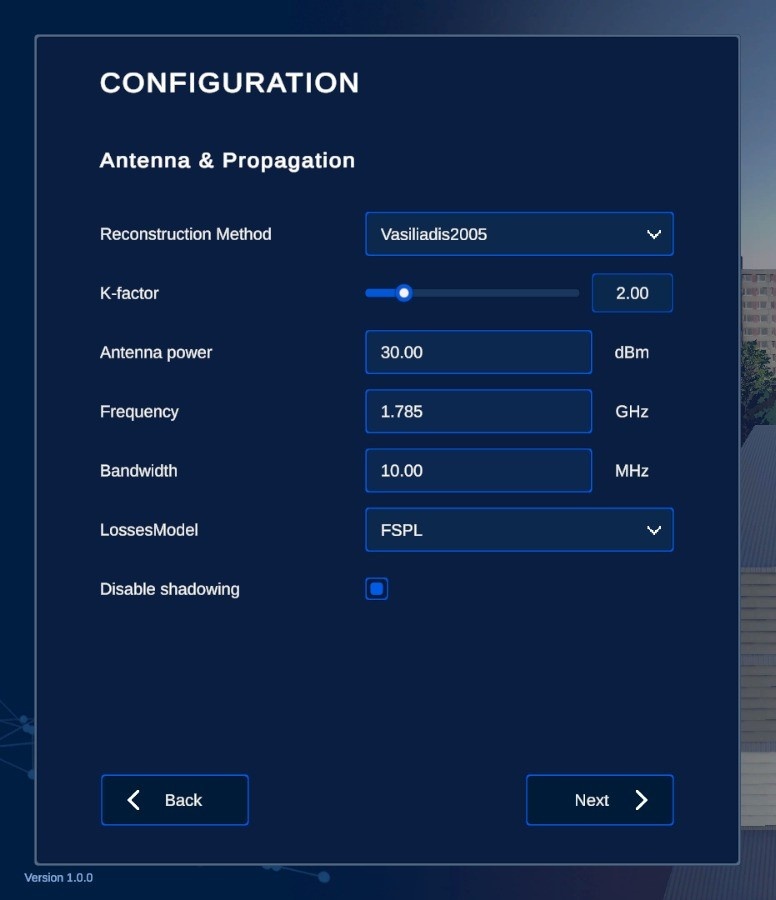
\includegraphics[width=0.75\textwidth, keepaspectratio]{imagenes/diseños/Diseño menu configuracion.jpeg}
    \caption{Diseño del menú de configuración}
    \label{fig:diseno_menu}
\end{figure}

El resto de pantallas siguen la misma idea de organización por bloques. La segunda pantalla permite configurar la rejilla de propagación y los receptores móviles, indicando las dimensiones del mapa de calor, el tamaño de cada vóxel y las ganancias de los receptores. La tercera pantalla agrupa las opciones de visualización y rendimiento, como la transparencia de los vóxeles o el modo de rendimiento de la aplicación. Por último, la cuarta pantalla de resultados y gráficas se utiliza para seleccionar qué gráficas se generarán para cada receptor móvil al finalizar la simulación.

En la pantalla de configuración de la rejilla se muestra también el número total de vóxeles que se generarán con los valores seleccionados. Esto sirve como referencia para que el usuario pueda estimar la carga de la simulación antes de iniciarla, ya que una rejilla más detallada aumenta el número de vóxeles que deben generarse y puede afectar al rendimiento según las características del equipo utilizado.

Antes de cargar la escena de simulación, la aplicación valida los valores introducidos por el usuario. Si algún parámetro no es correcto, no se permite continuar hasta que sea corregido. Una vez validada la configuración, los datos se guardan y se utilizan para inicializar la escena de simulación.

\section{Diseño de la escena de simulación}

La escena de simulación es la parte principal de la aplicación, ya que en ella se encuentran el escenario tridimensional, el patrón de radiación, los mapas de calor y los receptores móviles. Esta escena se carga después de validar la configuración del menú inicial.

La ejecución de la escena sigue el flujo mostrado en la Figura \ref{fig:flujo_ejecucion}. Nada más cargar la escena, el primer paso es cargar la configuración guardada en el menú. A continuación, se reconstruye el patrón de radiación de la antena y se prepara la rejilla de propagación sobre la que se calculará la potencia recibida. Posteriormente, se envían los datos a Python y una vez recibidos los resultados de la rejilla, se representan los mapas de calor. Finalmente, se activan los receptores móviles y, durante la simulación, sus métricas se actualizan y guardan periódicamente.

\begin{figure}[H]
    \centering
    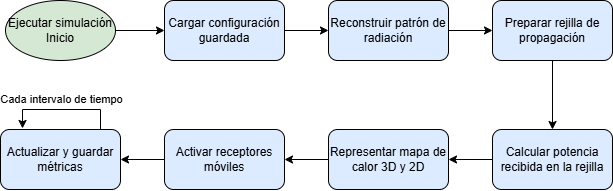
\includegraphics[width=1\textwidth, keepaspectratio]{imagenes/diagramas/Diagrama de flujo - ejecutar simulación.png}
    \caption{Flujo de ejecución de la simulación}
    \label{fig:flujo_ejecucion}
\end{figure}

Para representar la cobertura en el escenario, la aplicación crea una rejilla tridimensional de vóxeles. Un vóxel puede entenderse como el equivalente a un píxel, pero en tres dimensiones: en lugar de representar un punto de una imagen 2D, representa una región del espacio. Para cada vóxel se calcula un valor de potencia recibida y, a partir de ese valor, se colorea la región correspondiente dentro del mapa de calor.

Esta representación permite observar la distribución de potencia dentro de un volumen, pero también tiene una limitación importante. Cuando se muestran muchos vóxeles semitransparentes al mismo tiempo, la visualización puede saturarse y hacer que gran parte del escenario se vea con tonos similares. Por este motivo, se añaden parámetros de transparencia y un umbral de visualización. Las transparencias permiten controlar el peso visual de los vóxeles según su potencia, mientras que el umbral permite ocultar las zonas con menor potencia recibida y centrarse en las regiones más relevantes.

Además del mapa de calor 3D, se añade un minimapa 2D por capas, que permite analizar la misma información en cortes horizontales a distintas alturas. De esta forma, el usuario puede consultar tanto la distribución general de la potencia en el volumen como el comportamiento de una capa concreta. Por defecto, se muestra la capa más próxima a la altura de la antena.

La escena se organiza en varias vistas para evitar mostrar toda la información al mismo tiempo y facilitar la visualización. Las vistas disponibles son las siguientes:

\begin{itemize}
    \item \textbf{Vista del mapa de calor:} muestra la distribución de la potencia recibida en el escenario mediante mapas de calor.
    \item \textbf{Vista del patrón de radiación:} permite observar el patrón de radiación reconstruido de la antena transmisora.
    \item \textbf{Vistas de receptores móviles:} cada receptor móvil tiene una vista propia, en la que la cámara sigue su recorrido y se muestran sus métricas de enlace.
\end{itemize}

Para controlar estas vistas, se utiliza una cámara que cambia de posición según la vista en el modo activo. En las vistas del mapa de calor y del patrón de radiación, la cámara se sitúa alrededor de la antena y puede ajustarse mediante sliders de zoom, rotación y elevación. Estos controles permiten observar los resultados desde distintos ángulos. En las vistas de los receptores móviles, la cámara sigue al receptor seleccionado.

La Figura \ref{fig:vista_heatmap} muestra la vista del mapa de calor dentro de la escena de simulación. En ella se puede ver la distribución de los elementos principales de esta vista, como los controles de cámara, el minimapa, el slider de umbral, los botones de simulación y las opciones de rendimiento.

\begin{figure}[H]
    \centering
    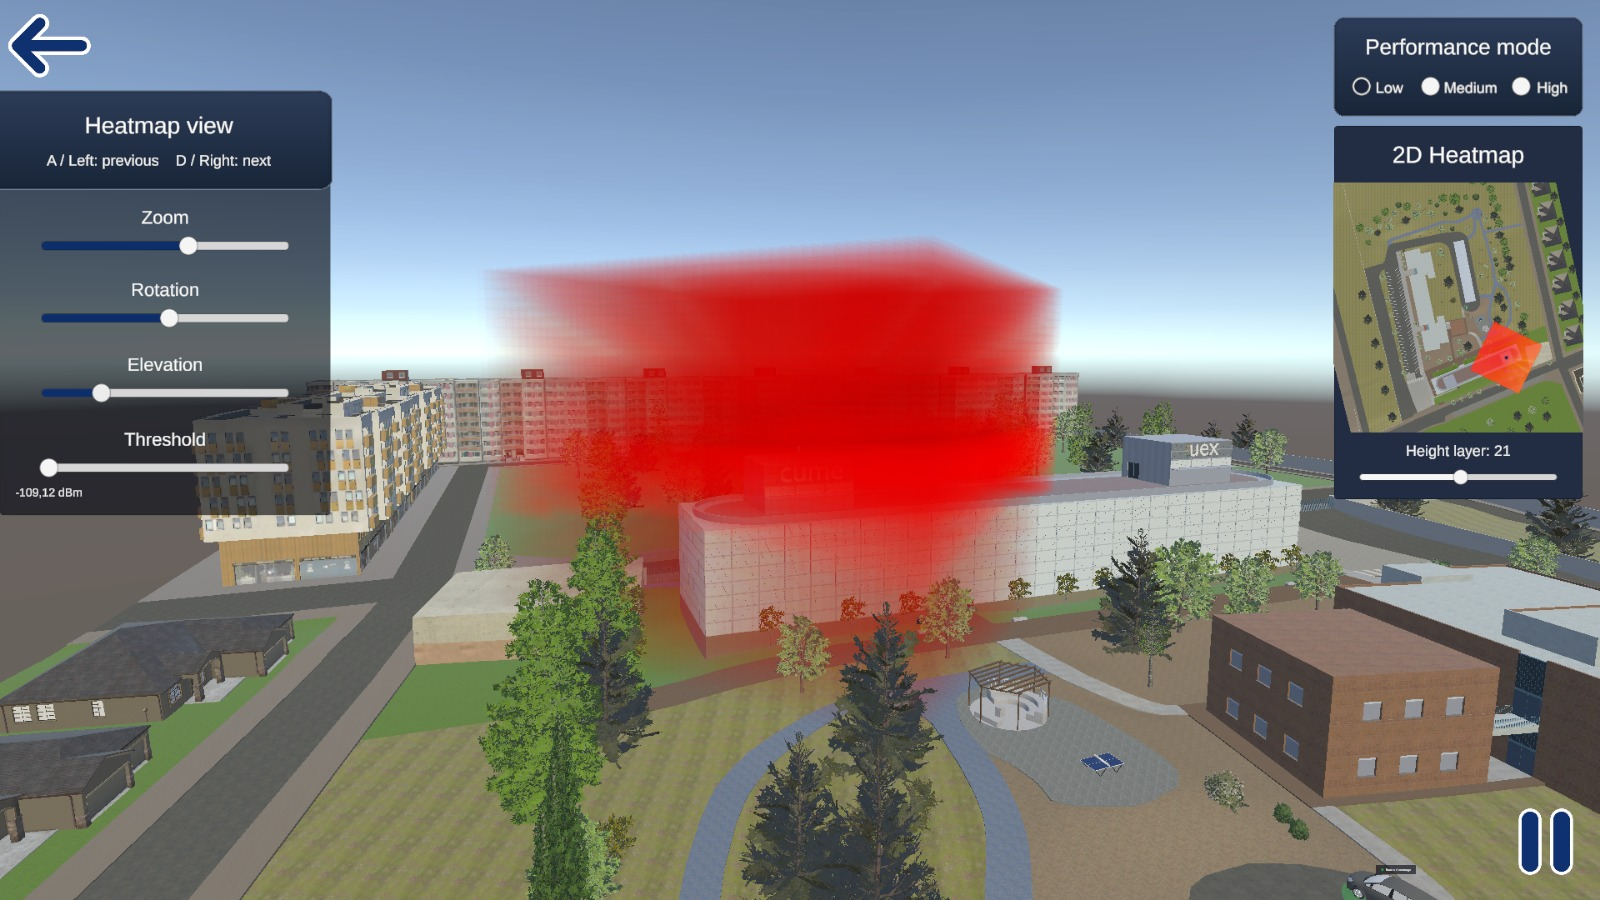
\includegraphics[width=1\textwidth, keepaspectratio]{imagenes/diseños/Diseño heatmapview.jpeg}
    \caption{Vista del mapa de calor}
    \label{fig:vista_heatmap}
\end{figure}

Además, el minimapa puede ampliarse al pulsar sobre él, mostrando la misma información con más detalle, como se observa en la Figura \ref{fig:minimapa_ampliado}. Esta vista ampliada también dispone de una leyenda con los valores mínimo y máximo de potencia recibida, lo que permite interpretar mejor la escala de colores utilizada en el mapa.

\begin{figure}[H]
    \centering
    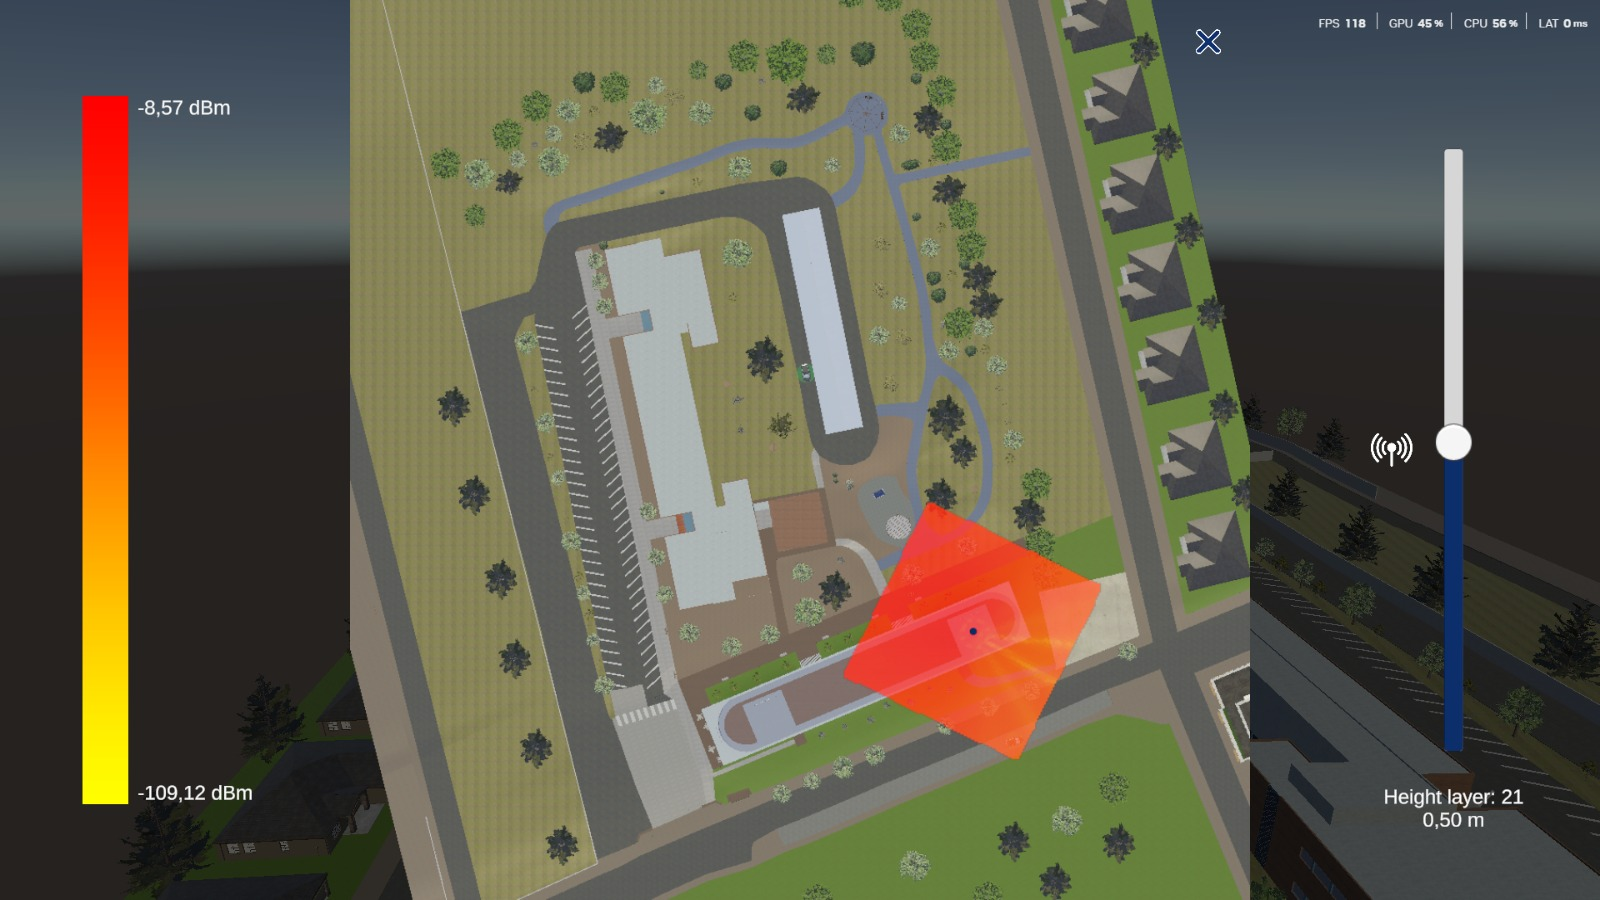
\includegraphics[width=1\textwidth, keepaspectratio]{imagenes/diseños/diseño minimapa ampliado.jpeg}
    \caption{Vista ampliada del minimapa 2D}
    \label{fig:minimapa_ampliado}
\end{figure}

La vista del patrón de radiación permite ver la forma tridimensional del patrón reconstruido, como se muestra en la Figura \ref{fig:vista_patron_radiacion}. Esta vista también incluye una leyenda con la ganancia mínima y máxima en dBi, de forma que el usuario pueda relacionar los colores y la forma del patrón con los valores de ganancia de la antena en cada dirección.

\begin{figure}[H]
    \centering
    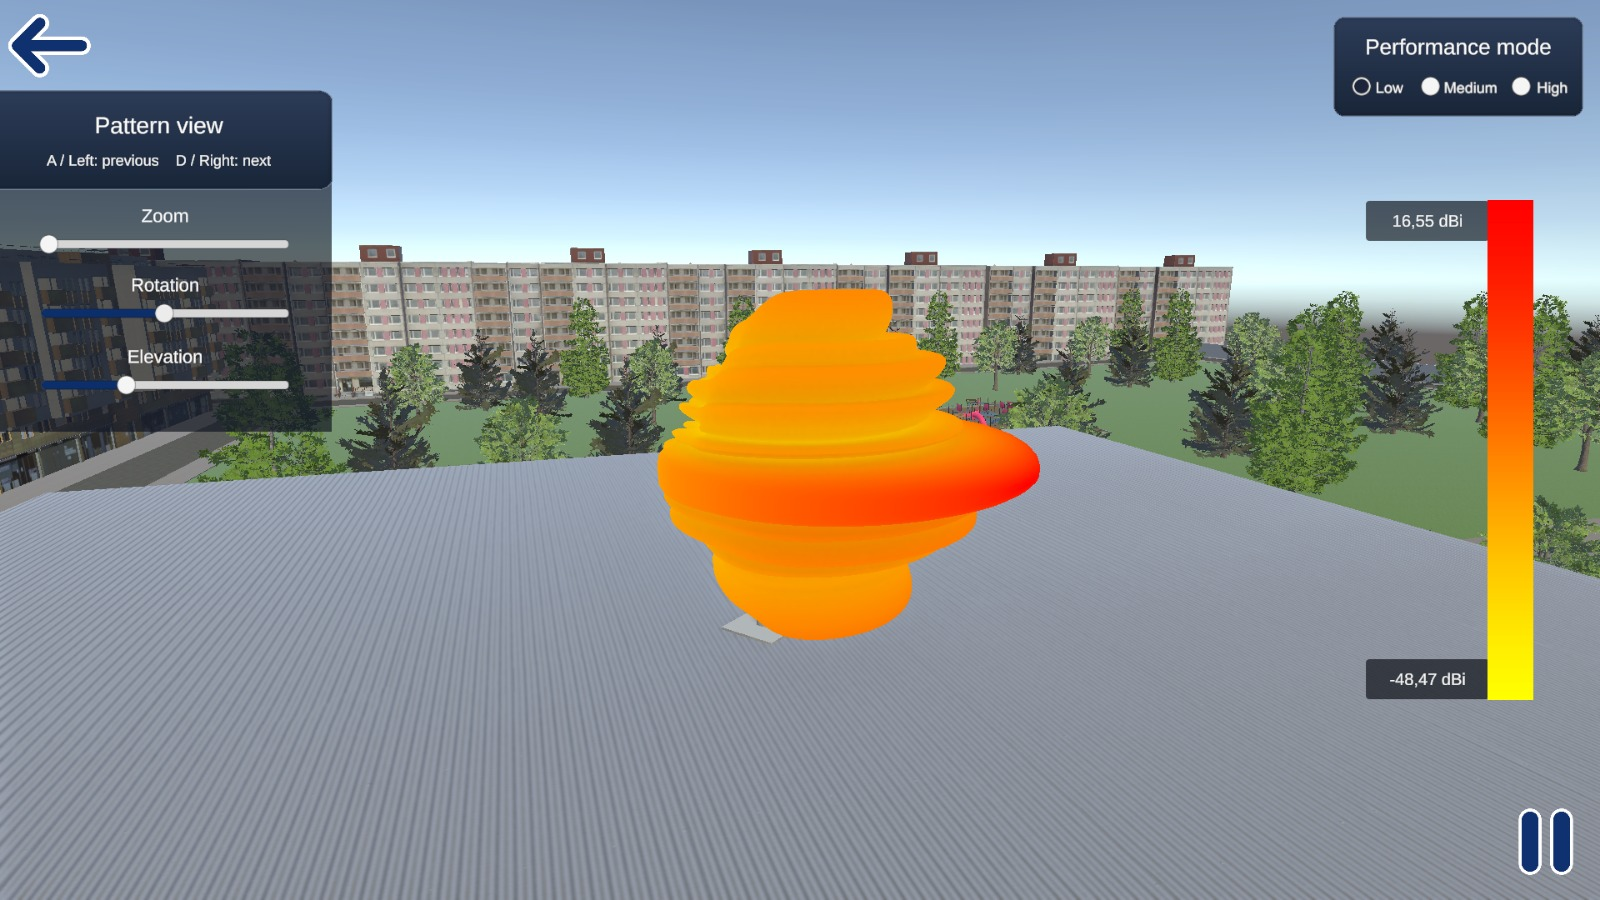
\includegraphics[width=1\textwidth, keepaspectratio]{imagenes/diseños/diseño pattern view.jpeg}
    \caption{Vista del patrón de radiación}
    \label{fig:vista_patron_radiacion}
\end{figure}

Las vistas de receptores móviles permiten seguir el recorrido de cada receptor dentro del escenario y ver sus métricas en tiempo real. En estas vistas, la cámara sigue al receptor seleccionado y se muestra un panel con información como la distancia al transmisor, la potencia recibida, la SNR, las pérdidas del enlace o las colisiones con edificios.

Además de las métricas numéricas, se añade a cada receptor móvil un indicador visual de cobertura. Este indicador muestra un mensaje sobre el receptor con el estado de la cobertura y un círculo de color en el suelo. De esta forma, se puede identificar rápidamente si la cobertura del receptor es excelente, buena, aceptable o insuficiente. En la Figura \ref{fig:vista_receptores} se muestra un ejemplo de vista asociada a un receptor móvil.

\begin{figure}[H]
    \centering
    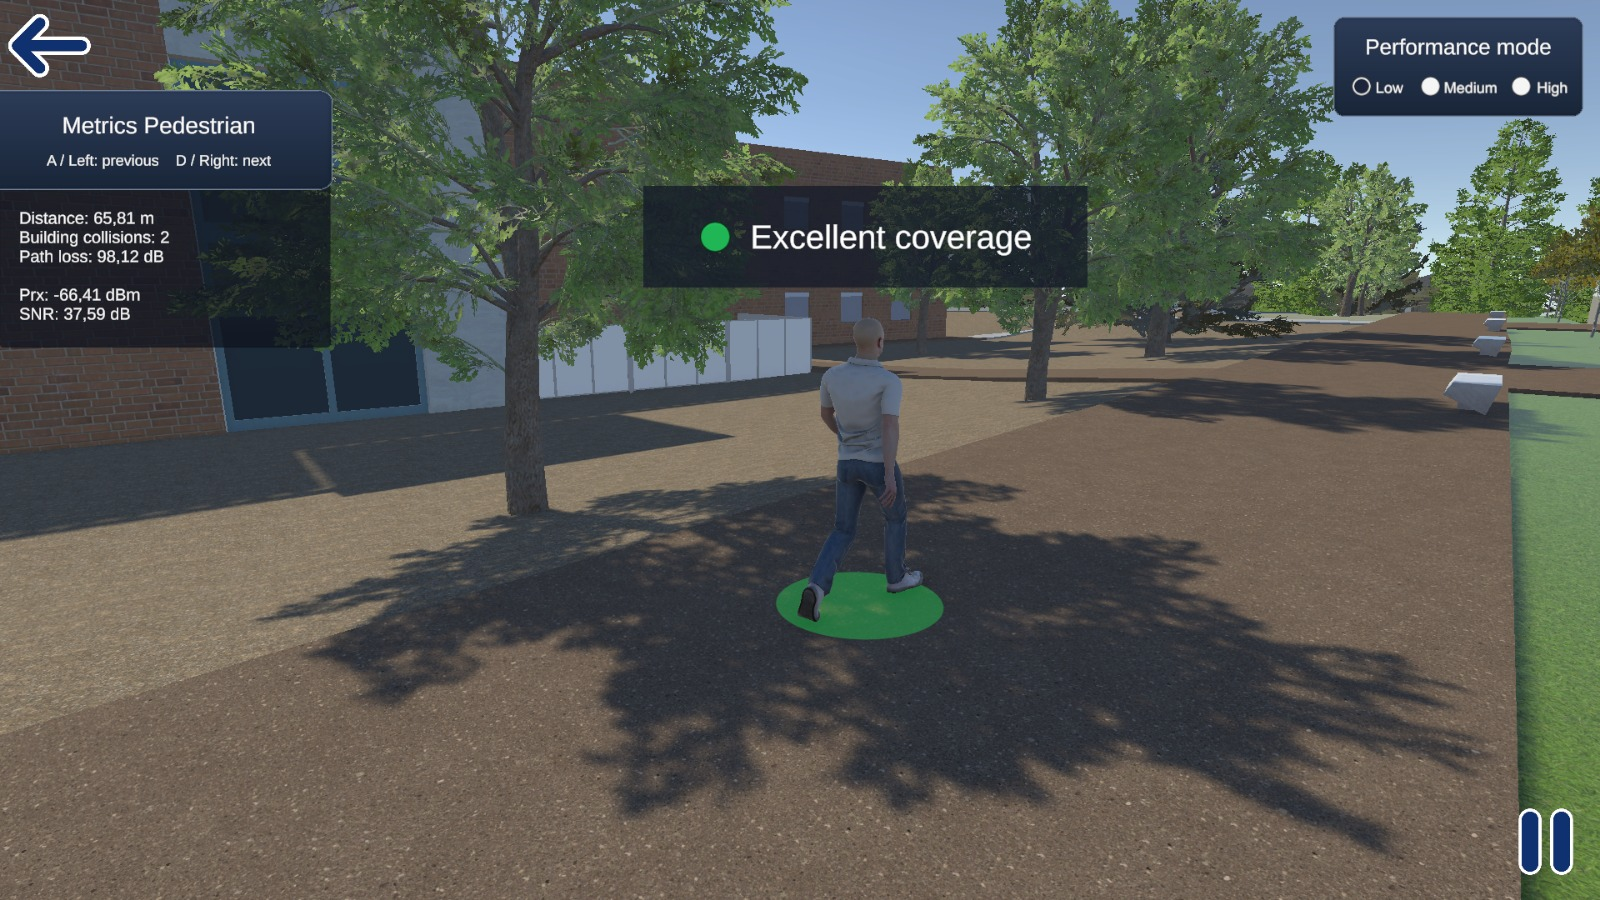
\includegraphics[width=1\textwidth, keepaspectratio]{imagenes/diseños/diseño receptores.jpeg}
    \caption{Vista de un receptor móvil}
    \label{fig:vista_receptores}
\end{figure}

La escena de simulación cuenta también con controles de simulación. En la parte inferior derecha, el botón de pausa permite detener la simulación, cambiando entre el icono de pausa y reanudar según el estado actual. El botón de volver al menú, en la parte superior izquierda, permite salir de la escena de simulación y volver al menú de configuración. Antes de volver, en caso de que queden resultados pendientes, la aplicación exporta los resultados para evitar que se pierdan los datos registrados hasta ese momento.

Por último, en la parte superior derecha se añaden botones de rendimiento. Estos permiten desactivar elementos secundarios del escenario, como vegetación, parque o edificios de fondo. Esta opción es clave para adaptar el simulador a equipos con diferentes prestaciones, ya que la representación del escenario y del mapa de calor puede afectar notablemente al rendimiento.


\section{Integración entre Unity y Python}

La integración entre Unity y Python permite reutilizar el simulador externo ya existente sin tener que reimplementar sus cálculos dentro de Unity. En este proyecto, Unity se encarga de la parte visual e interactiva de la aplicación, además de preparar los datos de la escena, como la rejilla y el patrón de radiación reconstruido. Por otro lado, Python se utiliza para integrar el simulador externo y realizar los cálculos del canal de propagación.

Para facilitar la ejecución de la aplicación, se incluye un entorno Python portable dentro del simulador. Este entorno contiene el intérprete de Python y las librerías necesarias para ejecutar el simulador externo y los scripts auxiliares, evitando que el usuario tenga que instalar Python o configurar dependencias de forma manual.

La comunicación entre ambos entornos se realiza de forma local mediante TCP. Unity actúa como cliente y Python como servidor. Cuando la escena de simulación necesita calcular la potencia recibida en la rejilla o actualizar las métricas de los receptores móviles, Unity prepara una petición y la envía al servidor Python. Una vez procesada, Python devuelve una respuesta con los resultados calculados.

Los mensajes intercambiados entre ambos entornos utilizan formato JSON. Esto permite enviar la información de forma estructurada y facilita la conversión de los datos entre C\# y Python, ya que ambos lenguajes disponen de librerías para serializar y deserializar datos en este formato. De esta forma, Unity puede generar una petición con los parámetros necesarios para la simulación y Python puede devolver una respuesta organizada con los valores obtenidos.


\section{Modelo de datos e intercambio de información}

Para que Unity y Python puedan intercambiar información, los datos se agrupan en Data Transfer Objects (DTO). Estos objetos son clases simples formadas por varios atributos y se utilizan para agrupar los datos que deben enviarse o recibirse en cada petición. Antes de enviar una petición, Unity convierte los DTO a JSON para poder transmitirlos al servidor Python. De la misma forma, cuando recibe una respuesta en JSON, la convierte a DTO para tratar los resultados de forma más sencilla dentro de la aplicación.

La Figura \ref{fig:intercambio_unity_python} muestra el intercambio de información entre Unity y Python para la rejilla de propagación y los receptores móviles.

\begin{figure}[H]
    \centering
    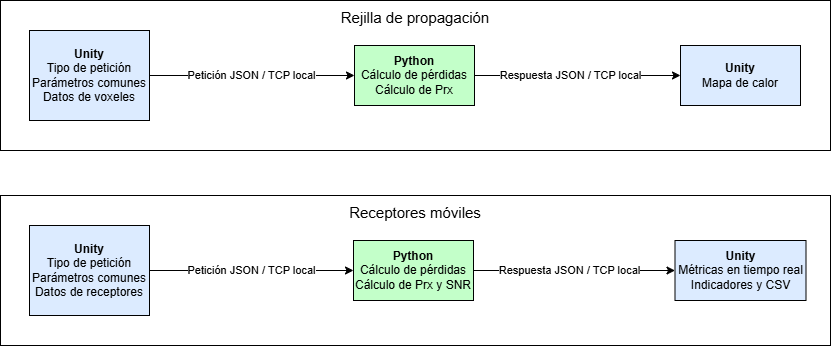
\includegraphics[width=1\textwidth, keepaspectratio]{imagenes/diagramas/Intercambio unity y python.png}
    \caption{Intercambio de información entre Unity y Python}
    \label{fig:intercambio_unity_python}
\end{figure}

En ambos casos, Unity envía una petición a partir de un DTO con parámetros comunes de la simulación, como la frecuencia o la potencia de transmisión, además de la información específica según el cálculo que se quiera realizar.

En el caso de la rejilla de propagación, Unity envía los datos de los vóxeles que forman el mapa de calor. Para cada vóxel se incluye su posición, la ganancia de transmisión correspondiente a esa dirección, el número de colisiones con edificios y la pérdida asociada. Python devuelve para cada punto la distancia al transmisor, las pérdidas del enlace y la potencia recibida. Con estos resultados, Unity colorea los vóxeles para representar el mapa de calor.

En el caso de los receptores móviles, Unity envía la posición actual de cada receptor, la ganancia de recepción y la ganancia de transmisión en la dirección transmisor-receptor. También se envía la información de colisiones y pérdidas asociadas. Python devuelve las métricas calculadas para cada receptor, entre ellas la potencia recibida y la SNR. Estos valores se utilizan para actualizar los paneles de métricas, los indicadores de cobertura y el registro de resultados.

\section{Diseño de la exportación de resultados}

La exportación de resultados se diseña para guardar la información generada durante la simulación y permitir su análisis posterior. Además de mostrar los resultados de forma visual dentro de Unity, el simulador genera archivos externos que pueden consultarse una vez finalizada la ejecución.

Los resultados se guardan dentro de una carpeta \texttt{Results} creada junto a la aplicación. Para cada ejecución se genera una subcarpeta identificada con la fecha y hora de la simulación. De esta forma, cada prueba queda separada del resto sin mezclar archivos generados en ejecuciones distintas.

Durante la simulación, la aplicación registra periódicamente las métricas de cada receptor móvil. Para cada muestra, se almacena el instante de tiempo, la distancia al transmisor, la posición del receptor, la potencia recibida, la SNR, las pérdidas del enlace y el número de colisiones con edificios. Estos datos se guardan posteriormente en archivos CSV, generando un fichero para cada receptor.

Estos CSV guardan todas las muestras obtenidas durante el recorrido. Esto permite reconstruir posteriormente el camino seguido por cada receptor, dibujar otro tipo de gráficas o analizar los datos con otros criterios fuera de la aplicación.

También se exporta un CSV con el patrón de radiación tridimensional reconstruido. Este archivo permite conservar la matriz de ganancias utilizada por el simulador para que pueda revisarse o analizarse fuera de Unity en caso de ser necesario.

Además, se guarda un fichero de configuración de la ejecución, donde se encuentran los parámetros principales utilizados en la simulación. Esto permite reconstruir posteriormente las condiciones de una prueba y comparar los resultados obtenidos con diferentes configuraciones.

A partir de los CSV, la aplicación permite generar gráficas automáticamente. Desde el menú de configuración, el usuario puede seleccionar qué gráficas quiere obtener para cada receptor, como potencia recibida frente a distancia, SNR frente a distancia o SNR frente al tiempo. Al finalizar la simulación, se utiliza el entorno Python integrado para generar estas gráficas a partir de los datos exportados.

Las gráficas frente a la distancia no se deben interpretar como una relación única entre distancia y cobertura, ya que en un escenario tridimensional existen muchos puntos distintos a una misma distancia del transmisor. La potencia recibida y la SNR también dependen de la dirección respecto al patrón de radiación, la altura, los obstáculos atravesados y el recorrido seguido por el receptor. Aun así, estas gráficas son útiles para comparar distintas configuraciones de simulación, patrones de antena o modelos de propagación bajo un mismo recorrido.

La exportación también se tiene en cuenta al volver al menú de configuración. Si el usuario sale de la escena de simulación y existen resultados pendientes, la aplicación los exporta antes de cargar de nuevo el menú.